\chapter{Θεωρητικό υπόβαθρο}\label{chapter:2-theoretical-background}

\section{Συναρτήσεις κατακερματισμού}

% Παλιό από Drive
Οι κρυπτογραφικές συναρτήσεις κατακερματισμού (cryptographic hash functions) είναι ειδική κατηγορία συναρτήσεων κατακερματισμού σχεδιασμένες για χρήση στην κρυπτογραφία. Οι συναρτήσεις κατακερματισμού είναι μαθηματικές συναρτήσεις που δέχονται ως είσοδο δεδομένα τυχαίου μεγέθους και επιστρέφουν συμβολοσειρές σταθερού μήκους αναπαράστασης.

% TODO: insert diagram

Οι τιμές που επιστρέφει η συνάρτηση κατακερματισμού ονομάζονται τιμές κατακερματισμού (hash values ή πιο απλά hashes). Μια ιδανική κρυπτογραφική συνάρτηση κατακερματισμού έχει τις εξής βασικές ιδιότητες:

\begin{itemize}
    \item Είναι ντετερμινιστική, έτσι η ίδια είσοδος παράγει πάντα την ίδια έξοδο.
    \item Ο υπολογισμός των hashes για οποιοδήποτε μήνυμα είναι γρήγορος.
    \item Δεν είναι εφικτό να βρεις την είσοδο από το hash, παρά μόνο δοκιμάζοντας όλα τα πιθανά μηνύματα.
    \item Μία μικρή αλλαγή στο μήνυμα επιφέρει τόσο μεγάλες αλλαγές στο νέο παραγόμενο hash ώστε να φαίνεται ασυσχέτιστο με το παλιό.
    \item Δεν είναι εφικτό να βρεθούν δύο διαφορετικές είσοδοι που δίνουν το ίδιο hash.
\end{itemize}

% TODO: insert diagram

\section{Ασύμμετρη κρυπτογραφία} \label{section:2-2-asymmetric-cryptography}

Η ασύμμετρη κρυπτογραφία (asymmetric cryptography) ή κρυπτογραφία δημόσιου κλειδιού (public-key cryptography) αποτελεί κρυπτογραφικό σύστημα που βασίζεται στη χρήση ενός ζεύγους κλειδιών (key pair), του \textit{δημόσιου} (public key) και του \textit{ιδιωτικού} (private key). Αυτά τα κλειδιά είναι μαθηματικά συνδεδεμένα ως εξής:

\begin{itemize}
	\item Το ιδιωτικό κλειδί δε μπορεί να προκύψει γνωρίζοντας το δημόσιό του
	\item Ό,τι κρυπτογραφηθεί από το ένα μπορεί να αποκρυπτογραφηθεί μόνο από το άλλο 
\end{itemize}
	
Η δημιουργία ενός ζεύγους κλειδιών επιτυγχάνεται μέσω μιας \textit{γεννήτριας κλειδιών} (\textenglish{key generation function}), η οποία χρησιμοποιεί ειδικούς αλγορίθμους (π.χ. RSA), δεχόμενη ως είσοδο έναν τυχαίο αριθμό. Από τα παραχθέντα κλειδιά, το δημόσιο γνωστοποιείται σε τρίτους, ενώ το ιδιωτικό παραμένει μυστικό.

\begin{figure}[H]
	\centering
	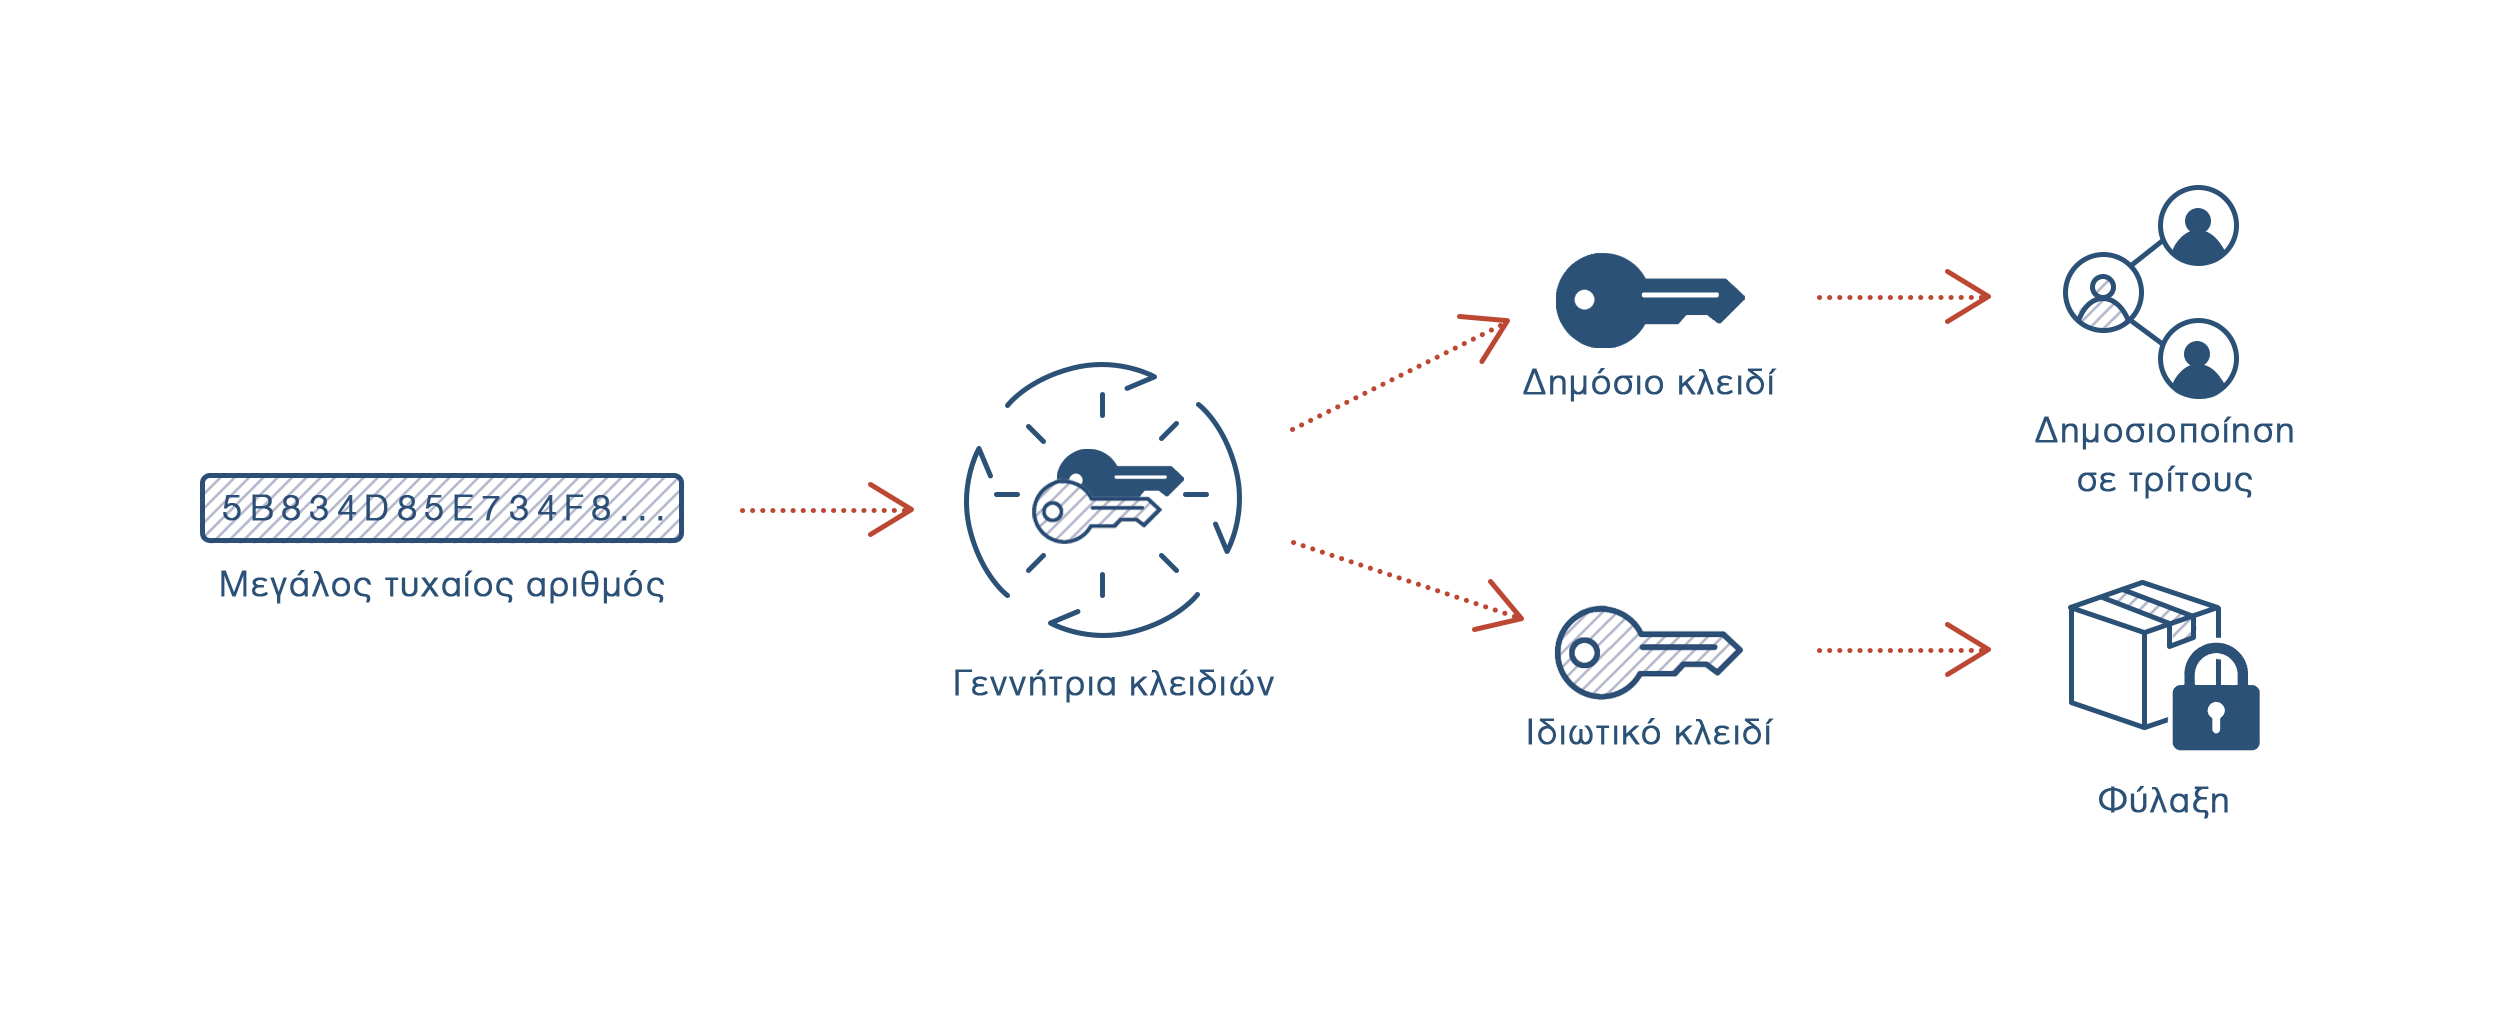
\includegraphics[width=.95\textwidth]{assets/figures/chapter-2/2.2.asymmetric-key-generation.png}
	\caption{Παραγωγή ασύμμετρου ζεύγους κλειδιών}
\end{figure}

Ο χρήστης μπορεί να χρησιμοποιήσει τα κλειδιά για δύο βασικούς σκοπούς:

\begin{enumerate}
	\item Για να αποκρυπτογραφήσει μηνύματα άλλων χρηστών, οι οποίοι τα κρυπτογράφησαν χρησιμοποιώντας το δημόσιο κλειδί του. Με αυτόν τον τρόπο εξασφαλίζεται η \textit{εμπιστευτικότητα} (confidentiality).
	\item Για να υπογράψει ψηφιακά ένα μήνυμα, κρυπτογραφώντας το hash των δεδομένων του με το ιδιωτικό του κλειδί. Έτσι, ο παραλήπτης του μηνύματος μπορεί μέσω της ληφθείσας \textit{ψηφιακής υπογραφής} (digital signature):
	\begin{enumerate}
		\item Να επαληθεύσει την ταυτότητα του αποστολέα, αποκρυπτογραφώντας επιτυχώς την ψηφιακή υπογραφή με το δημόσιο κλειδί του τελευταίου. Εξασφαλίζεται έτσι η \textit{πιστοποίηση} (authenticity) της προέλευσης των δεδομένων.
		\item Να επιβεβαιώσει ότι το μήνυμα έφτασε αναλλοίωτο, εφόσον το hash των δεδομένων συμπίπτει με το hash εντός της ψηφιακής υπογραφής. Με αυτόν τον τρόπο εξασφαλίζεται η \textit{ακεραιότητα} (integrity) των δεδομένων.
	\end{enumerate}
\end{enumerate}

Με τον συνδυασμό των παραπάνω, λέμε ότι δύο χρήστες μπορούν να επικοινωνούν μεταξύ τους με \textit{κρυπτογράφηση απ' άκρη σ' άκρη} (end to end encryption).

\begin{figure}[H]
	\centering
	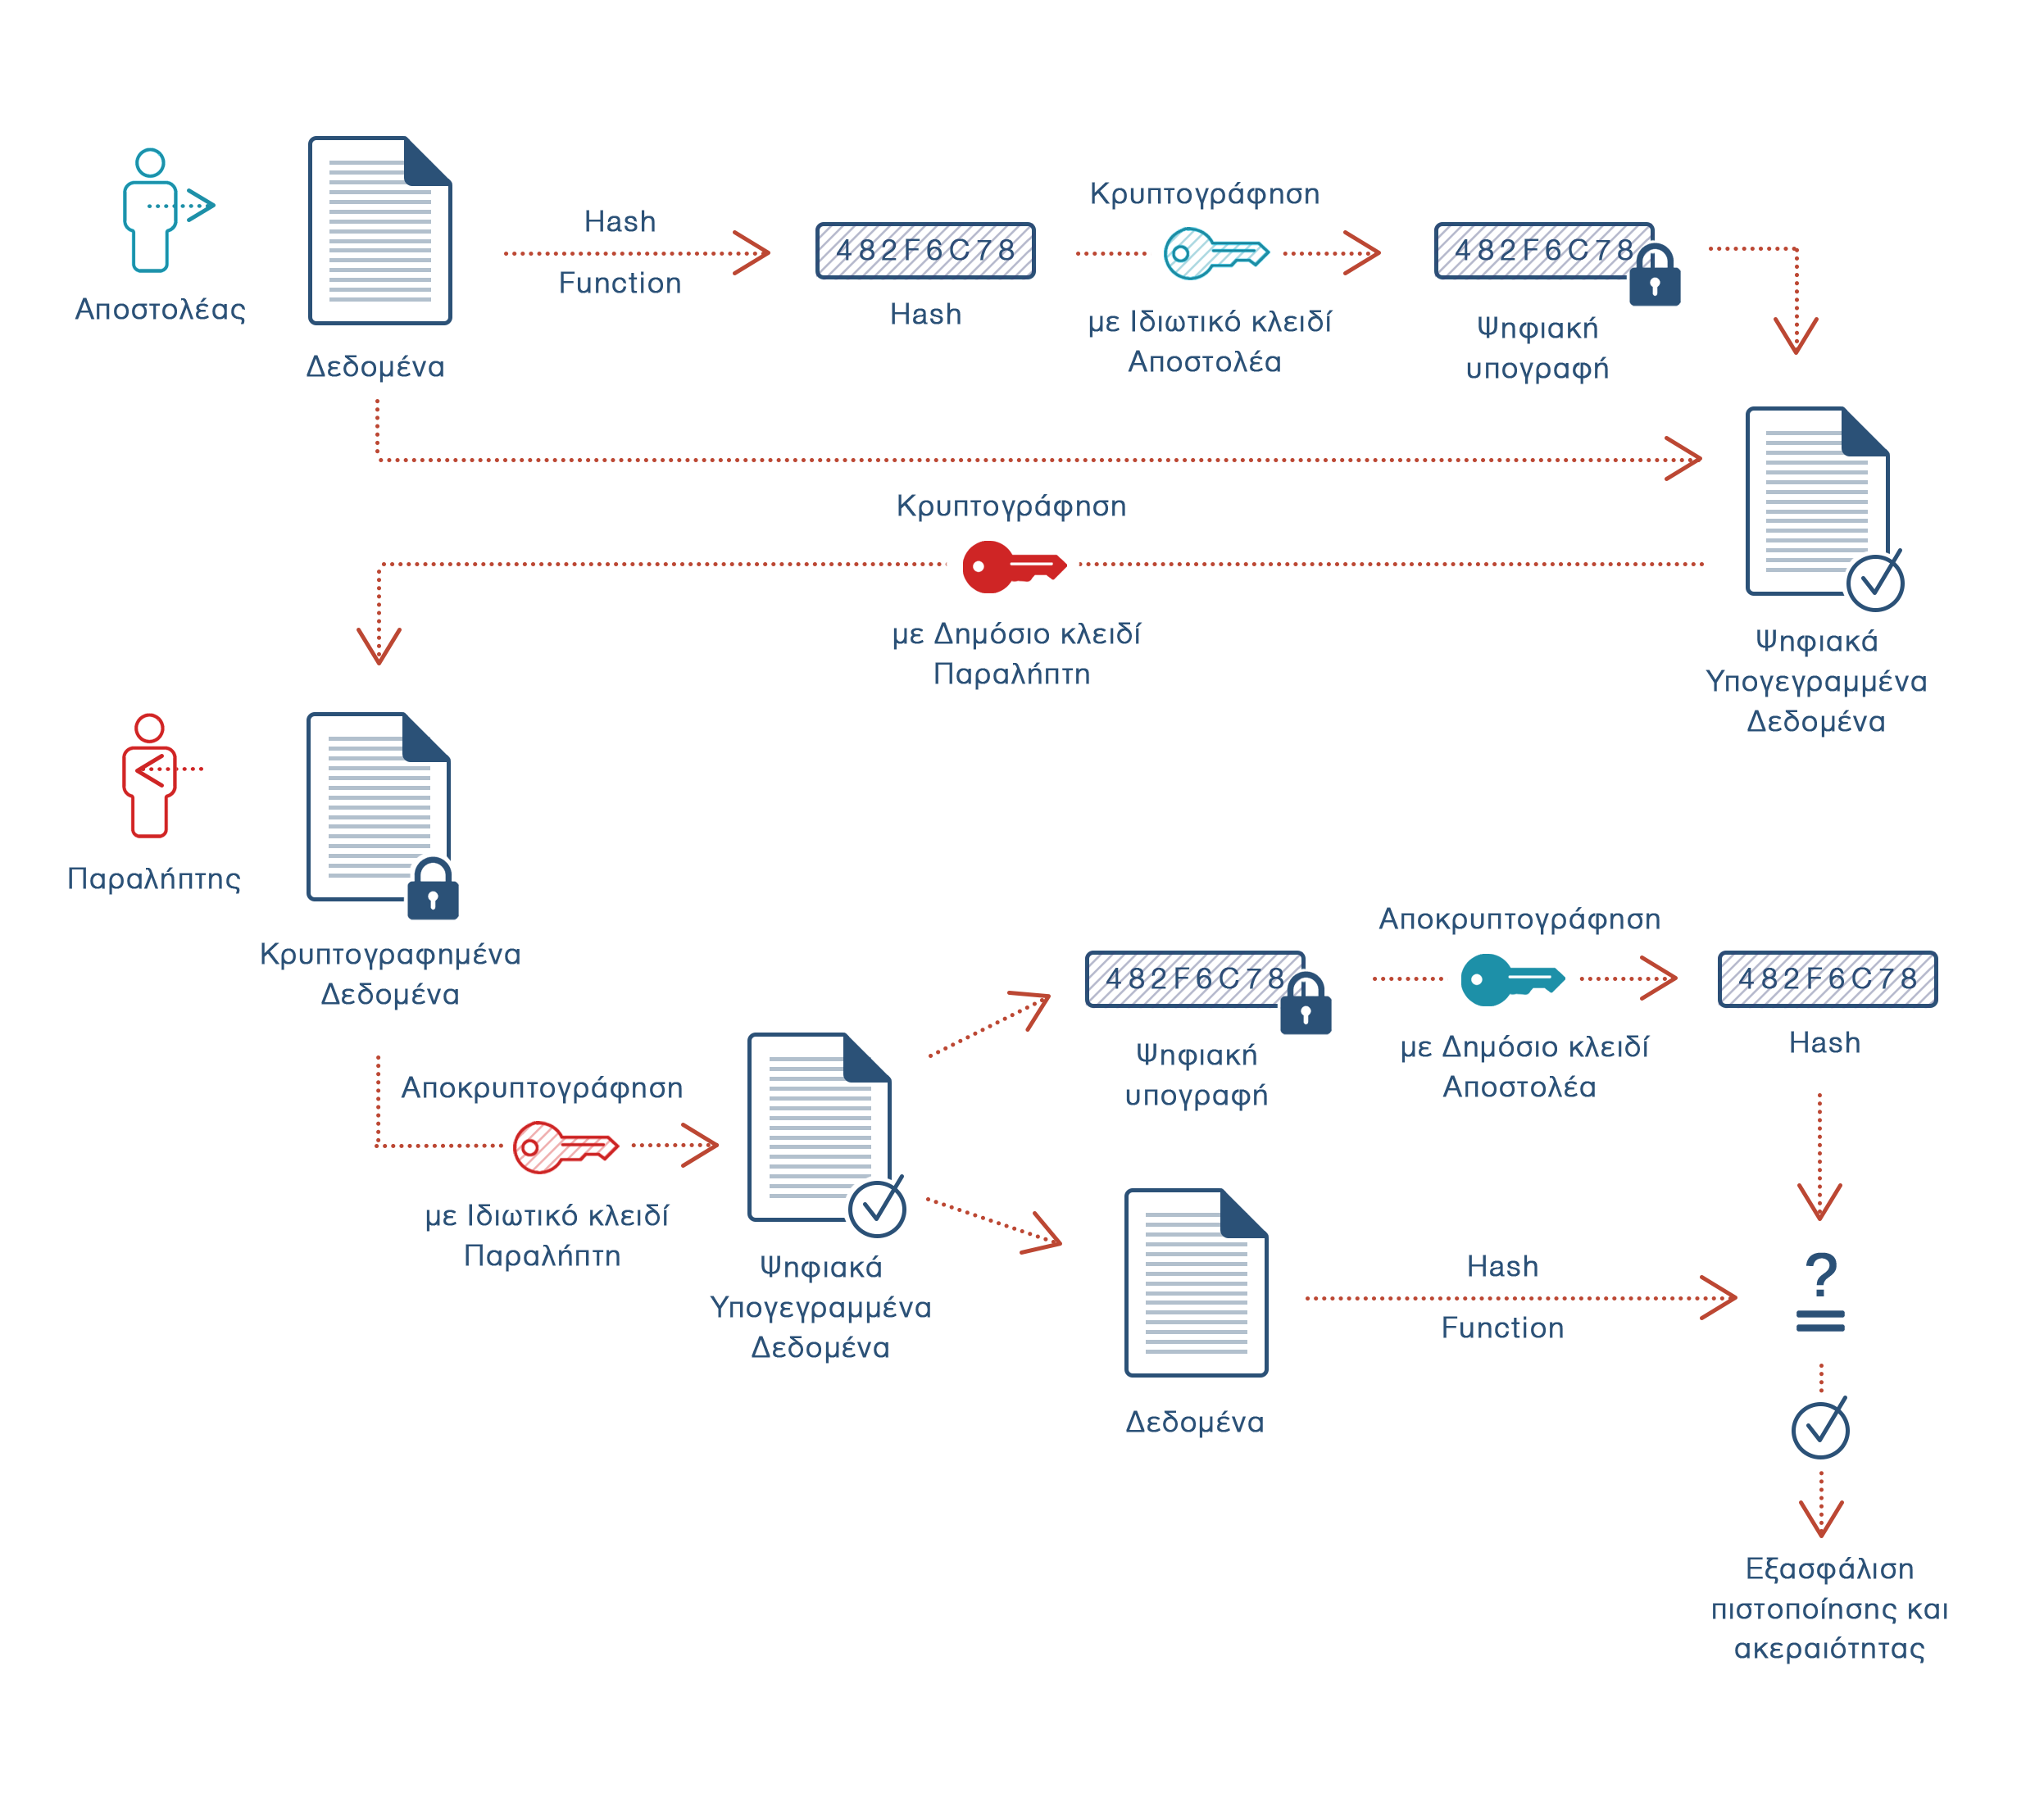
\includegraphics[width=.95\textwidth]{assets/figures/chapter-2/2.2.asymmetric-end-to-end-communication.png}
	\caption{Κρυπτογράφηση απ' άκρη σ' άκρη}
\end{figure}

 Μία προσέγγιση στην κρυπτογραφία δημόσιου κλειδιού είναι η κρυπτογραφία ελλειπτικής καμπύλης (Elliptic-Curve Cryptography ή ECC). Η ECC βασίζεται στην αλγεβρική δομή των ελλειπτικών καμπυλών σε πεπερασμένα πεδία και υπερέχει της non-EC κρυπτογραφίας, καθώς επιτρέπει τη δημιουργία μικρότερων κλειδιών με ισοδύναμη ασφάλεια. Ένα από τα πρωτόκολλά της είναι ο Elliptic Curve Digital Signature Algorithm (ECDSA), ο οποίος χρησιμοποιείται για την ψηφιακή υπογραφή δεδομένων και αποτελεί το EC-ανάλογο του DSA (Digital Signature Algorithm).\cite{2.2-ecdsa}
\section{Δένδρα Merkle} \label{section:2-3-merkle-trees}

Ένα δένδρο Merkle (Merkle tree ή hash tree) είναι μία δενδρική δομή δεδομένων, η οποία απαρτίζεται από φύλλα (leaf nodes) που περιέχουν hashes από blocks δεδομένων και από άλλους κόμβους (non-leaf nodes) που περιέχουν τα hashes των θυγατρικών τους. Στην κορυφή του δένδρου βρίσκεται ο ριζικός κόμβος με το λεγόμενο root hash.\cite{2.3-merkle-tree}

Η πιο συνηθισμένη υλοποίηση είναι το δυαδικό (binary) δένδρο Merkle, το οποίο περιλαμβάνει δύο θυγατρικούς κόμβους (child nodes) κάτω από κάθε γονικό (non-leaf) κόμβο, και είναι αυτό που αναλύεται στη συνέχεια.

\begin{figure}[H]
	\centering
	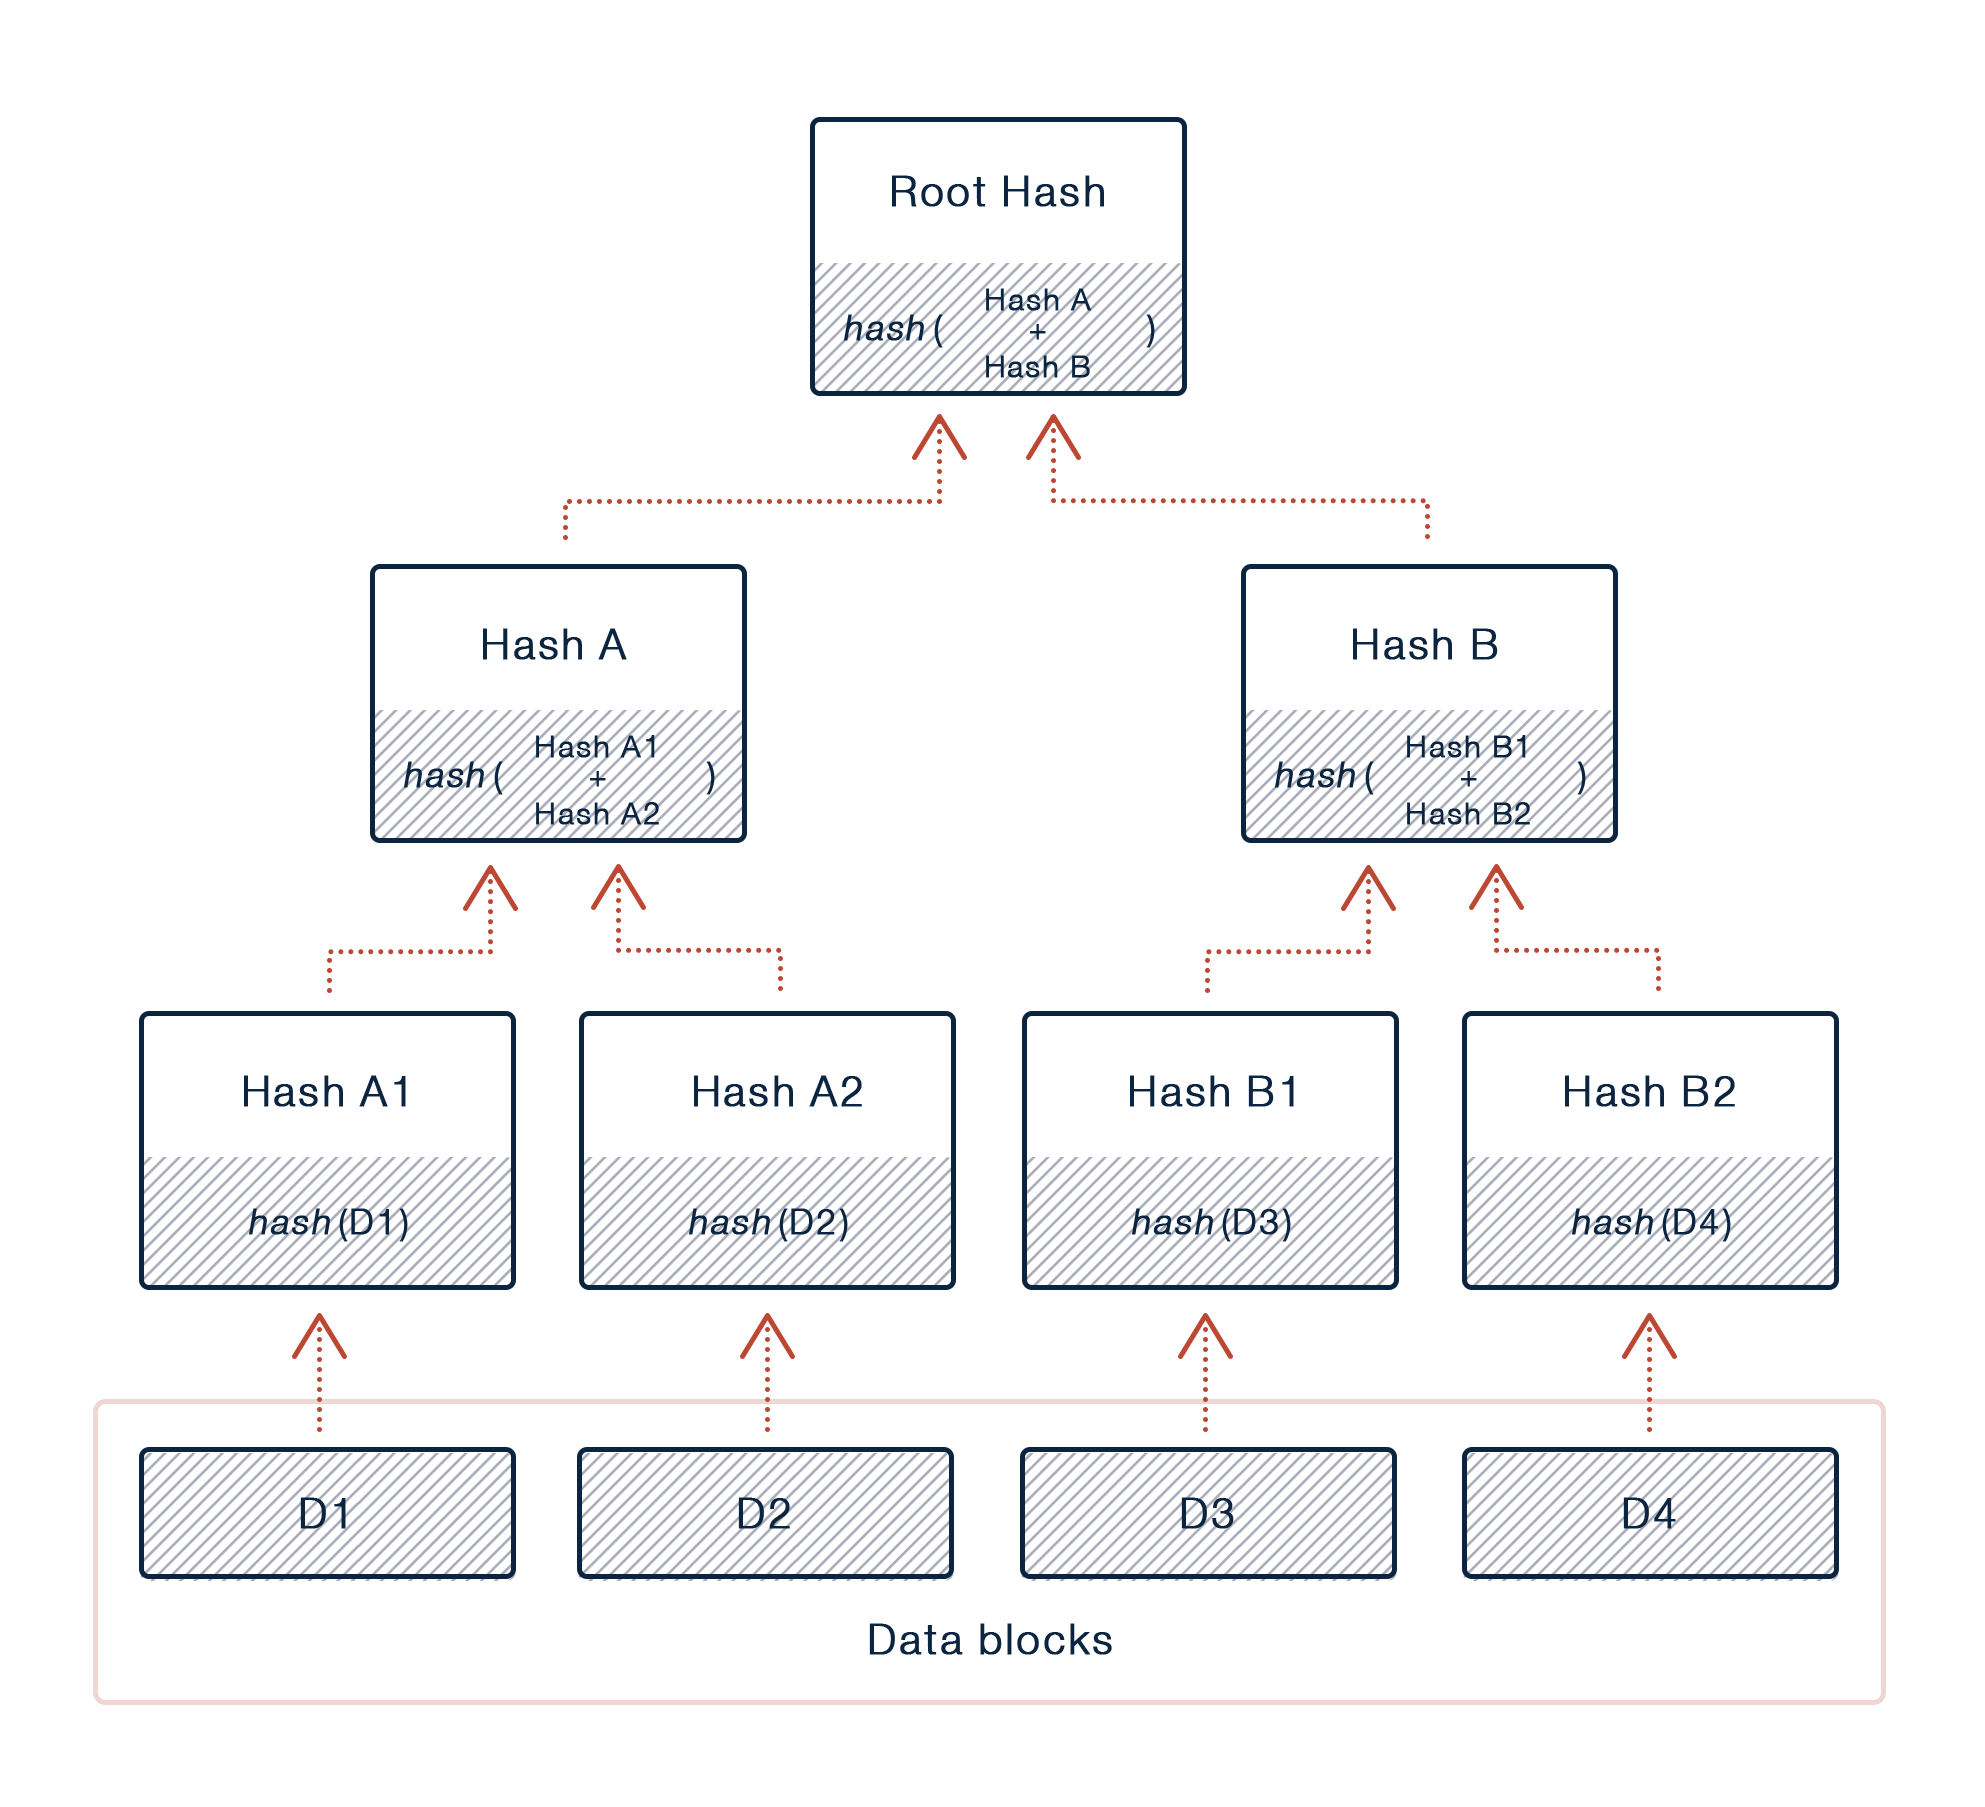
\includegraphics[width=.95\textwidth]{assets/figures/chapter-2/2.3.merkle-tree.png}
	\caption{Παράδειγμα δυαδικού δένδρου Merkle}
\end{figure}

Τα Merkle trees επιτρέπουν την αποδοτική και ασφαλή επαλήθευση των περιεχομένων που ανήκουν σε σετ δεδομένων μεγάλου μεγέθους. Η βασική ιδιότητα είναι ότι για κάθε σετ δεδομένων υπάρχει ακριβώς ένα πιθανό δένδρο, το οποίο δε γίνεται να τροποποιηθεί χωρίς να αλλάξει ταυτόχρονα και το root hash. 

Έτσι, μέσω των λεγόμενων Merkle proofs, μπορούμε:
\begin{itemize}
	\item Να αποφανθούμε εάν κάποια δεδομένα ανήκουν στο δένδρο, υπολογίζοντας (για το εκάστοτε leaf node) hashes πλήθους ανάλογου του λογαρίθμου του συνολοικού αριθμού των φύλλων.
	\item Να αποδείξουμε συνοπτικά την εγκυρότητα ενός τμήματος κάποιου σετ δεδομένων, χωρίς να χρειαστεί να αποθηκεύσουμε ολόκληρο το σύνολο δεδομένων.
	\item Να διασφαλίσουμε την εγκυρότητα ενός συγκεκριμένου συνόλου δεδομένων εντός ενός μεγαλύτερου σύνολου, χωρίς να χρειαστεί να αποκαλυφθεί το περιεχόμενο οποιουδήποτε εκ των δύο.\cite{2.3-merkle-proofs-explained} 
\end{itemize}

\section{Δίκτυα Ομότιμων Κόμβων}

Τα δίκτυα ομότιμων κόμβων ή Peer-to-Peer (P2P) networks αποτελούν μία κατανεμημένη αρχιτεκτονική δικτύων, οι συμμετέχοντες (κόμβοι) της οποίας μοιράζονται ένα τμήμα των πόρων τους, με στόχο την παροχή κάποιας υπηρεσίας (π.χ. τον διαμοιρασμό περιεχομένου). Εν αντιθέσει με συγκεντρωτικά δίκτυα τύπου client/server, οι κόμβοι (nodes) έχουν απευθείας πρόσβαση στους πόρους, χωρίς τη διαμεσολάβηση ενδιάμεσων οντοτήτων. Οι συμμετέχοντες ενός τέτοιου δικτύου είναι, δηλαδή, ταυτόχρονα, τόσο πάροχοι, όσο και αιτούντες των πόρων και της παρεχόμενης υπηρεσίας.\cite{p2p-networking}

Τα P2P networks μπορούν να χωριστούν σε δύο κατηγορίες:

\begin{itemize}
	\item Στα "Καθαρά" (Pure) P2P networks, στα οποία ισχύει ότι η αφαίρεση ενός τυχαίου κόμβου από το δίκτυο δεν προκαλεί κάποιο πρόβλημα σε αυτό.
	\item Στα "Υβριδικά" (Hybrid) P2P networks, στα οποία συμμετέχουν επιπλέον και κεντρικές οντότητες, παρέχοντας απαραίτητα τμήματα των προσφερόμενων υπηρεσιών.
\end{itemize}

Από εδώ και στο εξής, εάν δεν αναφέρεται ρητά η κατηγορία κάποιου P2P network, θα εννοείται ότι ανήκει στην πρώτη.


\section{Blockchain} \label{section:2-5-blockchain}

Το blockchain αποτελεί μία διανεμημένη δημόσια σειρά δεδομένων, που διατηρεί έναν αμετάβλητο ως προς το ιστορικό του κατάλογο (immutable ledger) ψηφιακών συναλλαγών (digital transactions) ενός αγαθού (asset), π.χ. ενός νομίσματος (currency ή token). Περιγράφηκε για πρώτη φορά το 2008 από ένα άτομο (ή μία ομάδα ανθρώπων) με το ψευδώνυμο Satoshi Nakamoto, αποτελώντας τη βάση του κρυπτονομίσματος (cryptocurrency) Bitcoin.\cite{2.5-bitcoin}

Δομικό στοιχείο του blockchain είναι το μπλοκ (block), το οποίο περιέχει μία ομάδα έγκυρων συναλλαγών που έχουν κατακερματιστεί και κωδικοποιηθεί σε ένα δένδρο Merkle, το hash του προηγούμενου μπλοκ και μερικά ακόμα μεταδεδομένα (π.χ. nonce, timestamp). Έτσι, κάθε νέο μπλοκ "δείχνει" στο προηγούμενό του μέσω του hash, επιβεβαιώνοντας την ακεραιότητά του, με τα διαδεχόμενα μπλοκ να σχηματίζουν τελικά μία αλυσίδα, μέχρι το αρχικό μπλοκ, το οποίο είναι γνωστό ως το μπλοκ γένεσης (genesis block).

\vspace{.5\baselineskip}

\begin{figure}[H]
	\centering
	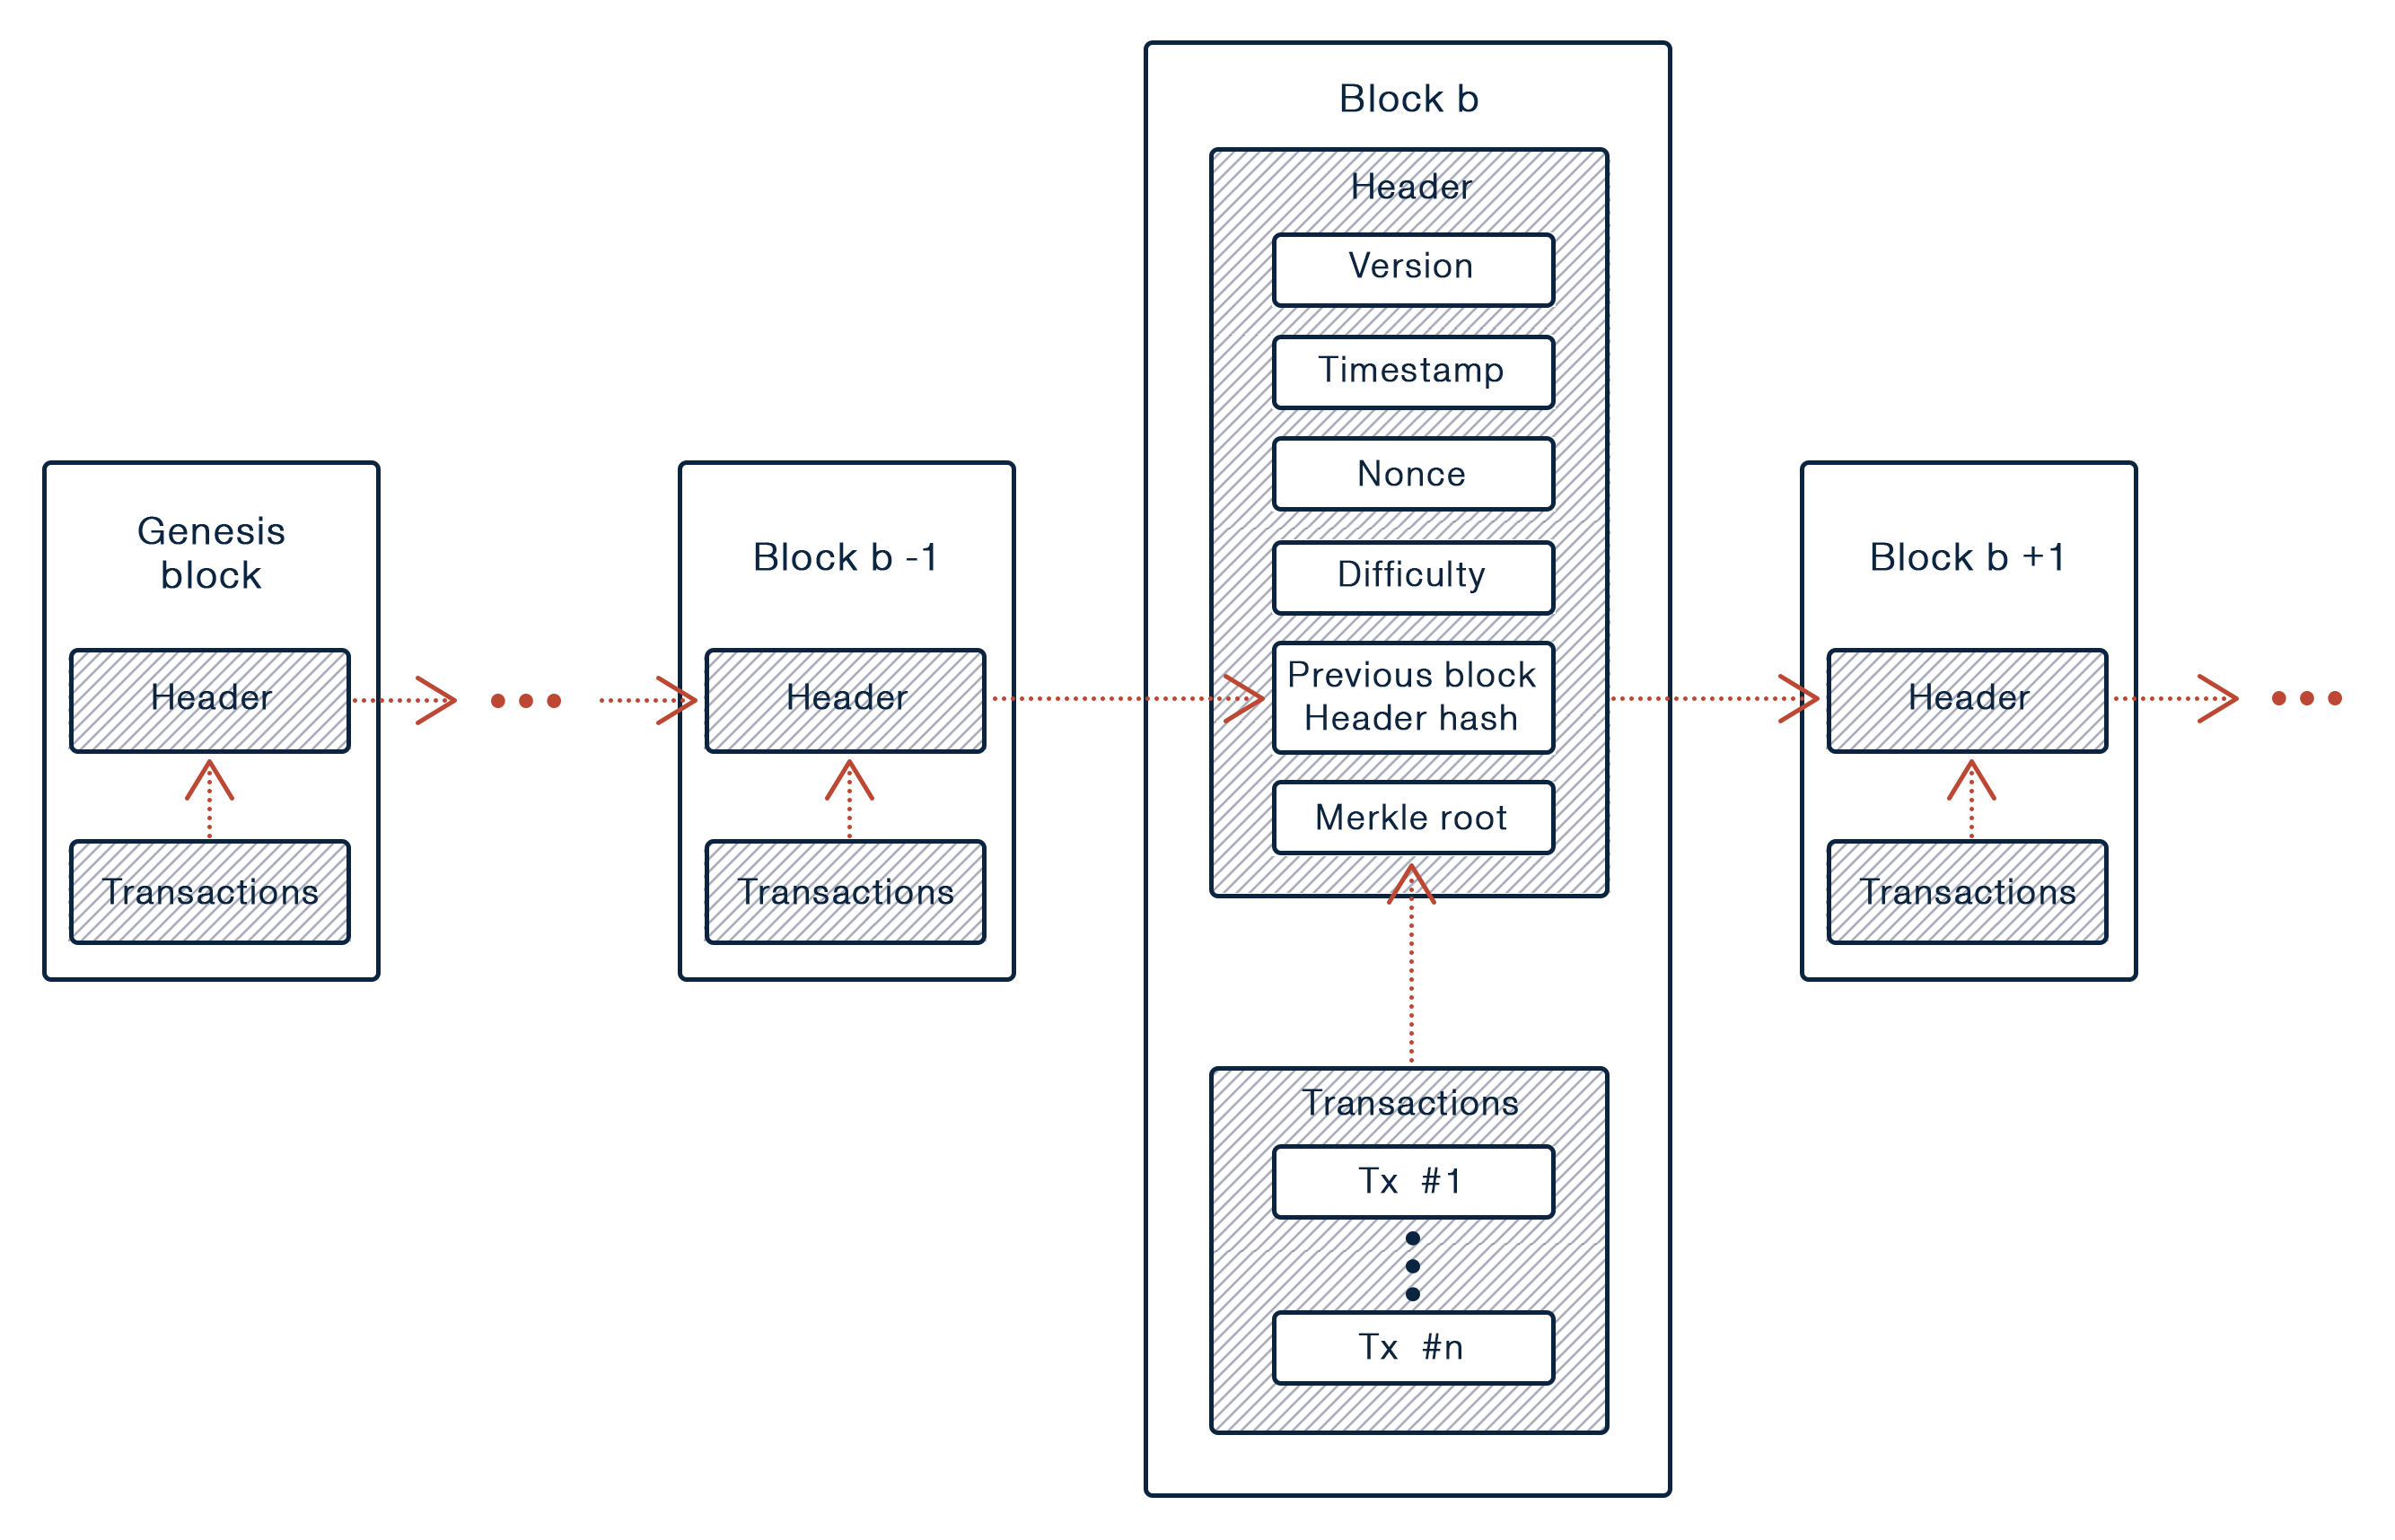
\includegraphics[width=.95\textwidth]{assets/figures/chapter-2/2.3.blockchain}
	\caption{Blockchain ως αλυσίδα από block}
\end{figure}

\vspace{.5\baselineskip}

Ως προς την κυριότητα επί αυτού, το blockchain συνήθως\footnote{Υπάρχουν και κάποιες υλοποιήσεις ιδιωτικών blockchain που, όμως, δε θα μας απασχολήσουν.} δεν ελέγχεται από κάποια κεντρική οντότητα, αλλά διατηρείται από ένα δημόσιο P2P δίκτυο. Οι κόμβοι του δικτύου συμμορφώνονται συλλογικά με ένα πρωτόκολλο συναίνεσης (consensus) για την επικοινωνία και την επικύρωση νέων μπλοκ. Για παράδειγμα, στο Bitcoin, το consensus επιτυγχάνεται μέσω ενός Proof of Work (PoW) αλγορίθμου, όπου οι κόμβοι (miners) ανταγωνίζονται ο ένας τον άλλον για το ποιος θα λύσει πρώτος ένα σύνθετο αλγοριθμικό πρόβλημα που συσχετίζεται με το εκάστοτε block. Αυτός που θα τα καταφέρει επιβραβεύεται για την επεξεργαστική ισχύ που δαπάνησε με ένα ποσό από bitcoin. Εκείνα είναι εν μέρει νέα νομίσματα που κόβονται ή "εξορύσσονται" εκείνη τη στιγμή (όπως ορίζεται από το πρωτόκολλο), αλλά και όσα τέλη (fees) κατέβαλαν οι κόμβοι για να πραγματοποιήσουν τις συναλλαγές του μπλοκ. Αξίζει να σημειωθεί πως δεν είναι αναγκαίο να διαθέτει κανείς ολόκληρο το blockchain (το οποίο είναι ιδιαίτερα ογκώδες) - δηλαδή έναν πλήρη κόμβο - για να επικοινωνήσει με το δίκτυο, αλλά αρκεί να χρησιμοποιήσει έναν light node που απλά να αναμεταδίδει τις επιθυμητές συναλλαγές.

Η διευθυνσιοδότηση σε ένα blockchain επιτυγχάνεται αξιοποιώντας την κρυπτογραφία δημόσιου κλειδιού. Το πρωτόκολλο του εκάστοτε blockchain ορίζει έναν αλγόριθμο για την παραγωγή ζευγών κλειδιών (π.χ. ECDSA στο Bitcoin). Το δημόσιο από αυτά ορίζει τη διεύθυνση, ενώ το ιδιωτικό παραμένει μυστικό, υπό την κατοχή του χρήστη. Με αυτό τον τρόπο προκύπτει ένα πρακτικά ανεξάντλητο πλήθος πιθανών έγκυρων δημόσιων διευθύνσεων (π.χ. $2^{160}$ για το Bitcoin), στις οποίες οι χρήστες μπορούν να στέλνουν και να λαμβάνουν ποσά του εκάστοτε κρυπτονομίσματος. Για την αποστολή ενός ποσού, δηλώνουν το fee που επιθυμούν να καταβάλουν και υπογράφουν την επιθυμητή συναλλαγή με το ιδιωτικό τους κλειδί. Η συναλλαγή αναμεταδίδεται στο δίκτυο και παραμένει στο transaction pool μέχρις ότου να γίνει αποδεκτή και να συμπεριληφθεί στο επόμενο block.

Από τεχνική σκοπιά, το blockchain μπορεί να θεωρηθεί ως μία μηχανή καταστάσεων βασισμένη σε συναλλαγές (transaction-based state machine). Δηλαδή, ξεκινάει από μία αρχική κατάσταση (genesis state), η οποία τροποποιείται σταδιακά με κάθε block, και περιλαμβάνει ανά πάσα στιγμή τις διευθύνσεις με τα ποσά των νομισμάτων που τις αντιστοιχούν.

\begin{figure}[H]
	\centering
	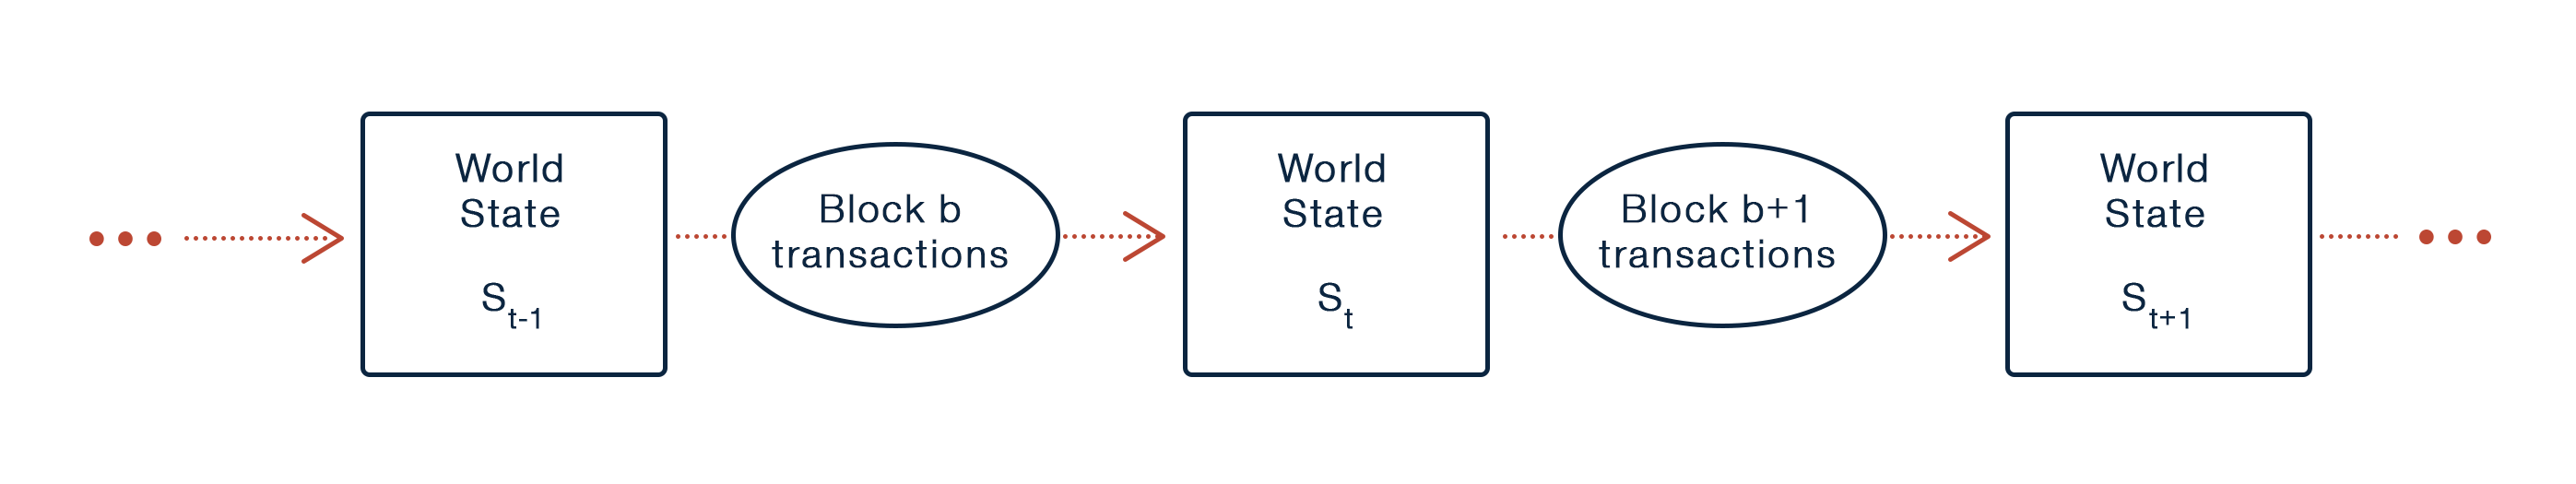
\includegraphics[width=.95\textwidth]{assets/figures/chapter-2/2.3.blockchain.world.state}
	\caption{Blockchain ως μηχανή καταστάσεων}
\end{figure}

Σύμφωνα με την ανάλυση της ενότητας \ref{section:1-2-decentralization}, το blockchain είναι αρχιτεκτονικά και πολιτικά αποκεντρωτικό, καθώς δε διαθέτει δομικά κάποιο κεντρικό σημείο αποτυχίας, ούτε ελέγχεται από κάποιον. Ωστόσο, είναι λογικά συγκεντρωτικό, αφού υπάρχει μία κοινά αποδεκτή κατάσταση και το σύστημα συμπεριφέρεται μακροσκοπικά ως ένας ενιαίος υπολογιστής.

\section{Ethereum} \label{section:2-6-ethereum}

\begin{figure}[H]
	\centering
	
\includegraphics[width=2cm]{assets/figures/ethereum-logo.png}
	\caption{Ethereum logo}
\end{figure}

Το Ethereum είναι ένα δημόσιο blockchain ανοιχτού κώδικα με εγγενές κρυπτονόμισμα το Ether (ETH). Παρέχει μία προγραμματιστική πλατφόρμα με ενσωματωμένη μία Turing-complete γλώσσα προγραμματισμού, που μπορεί να χρησιμοποιηθεί για τη δημιουργία αποκεντρωμένων εφαρμογών (Decentralized Applications ή DApps) μέσω της χρήσης "έξυπνων συμβολαίων" (smart contracts).\cite{2.6-ethereum-whitepaper}

\subsection{Λογαριασμοί} \label{subsection:2-6-1-ethereum-accounts}
Στο Ethereum blockchain οι λογαριασμοί αποτελούν οντότητες οι οποίες μπορούν να δέχονται, να κρατούν και να στέλνουν ETH και tokens, καθώς και να αλληλεπιδρούν με smart contracts.\cite{2.6-ethereum-documentation} Χωρίζονται σε δύο κατηγορίες: στους λογαριασμούς εξωτερικής κατοχής (\textenglish{externally owned accounts} ή EOAs) και στους λογαριασμούς συμβολαίων (contract accounts).

Οι λογαριασμοί εξωτερικής κατοχής δημιουργούνται χωρίς κόστος και ελέγχονται μέσω ιδιωτικών κλειδιών. Μπορούν να πραγματοποιούν μόνο συναλλαγές μεταφοράς ETH ή κάποιου token.

Από την άλλη, οι λογαριασμοί συμβολαίων απαιτούν κάποιο κόστος δημιουργίας, καθώς χρησιμοποιούν αποθηκευτικό χώρο επί του blockchain, ενώ ελέγχονται αποκλειστικά από τον κώδικά τους. Οι συναλλαγές που πραγματοποιούν προς άλλους λογαριασμούς είναι μόνο σαν αντίδραση σε μία εισερχόμενη συναλλαγή, όπως ορίζει ο κώδικας του smart contract τους.

Πιο αναλυτικά, τα πεδία που διαθέτουν οι λογαριασμοί στο Ethereum είναι τα εξής:

\begin{itemize}
	\item Το \textbf{nonce}: ένας μετρητής που υποδεικνύει τον αριθμό των απεσταλμένων συναλλαγών του λογαριασμού. Αυτό διασφαλίζει ότι οι συναλλαγές διεκπεραιώνονται μόνο μία φορά. Σε έναν λογαριασμό συμβολαίου, αυτός ο αριθμός αντιπροσωπεύει τον αριθμό των συμβολαίων που δημιουργήθηκαν από εκείνον.

	\item Το \textbf{balance}: το ποσό σε ETH που διαθέτει ο λογαριασμός, μετρημένο σε wei (1 ETH = $10^{18}$ wei).

	\item Το \textbf{codeHash}: ένα hash που αναφέρεται στον κώδικα του λογαριασμού (contract code). Είναι χαρακτηριστικό των λογαριασμών συμβολαίων (στους λογαριασμούς εξωτερικής κατοχής είναι hash μίας κενής συμβολοσειράς) και, σε αντίθεση με τα άλλα πεδία, αφότου οριστεί παραμένει αμετάβλητο.

	\item Το \textbf{storageRoot}: το root hash του δένδρου Merkle των αποθηκευμένων δεδομένων του smart contract, εφόσον πρόκειται για έναν λογαριασμό συμβολαίου (δε χρησιμοποιείται σε λογαριασμούς εξωτερικής κατοχής).
\end{itemize}

Η δημιουργία των λογαριασμών επιτυγχάνεται μέσω της παραγωγής ενός ζεύγους κλειδιών, αξιοποιώντας τον 
ECDSA (βλ. ενότητα \ref{section:2-2-asymmetric-cryptography}). Έτσι, το ιδιωτικό κλειδί χρησιμοποιείται για να υπογράφονται ψηφιακά οι συναλλαγές, ενώ το δημόσιο ορίζει τη δημόσια διεύθυνση του λογαριασμού (είναι της μορφής "0x + τα 20 τελευταία bytes του Keccak-256\footnote{Ο Keccak-256 αποτελεί τον κρυπτογραφικό αλγόριθμο κατακερματισμού που χρησιμοποειίται στο Ethereum. Πρόκειται για τον αλγόριθμο SHA3-256 πριν την τυποποίησή του από το NIST.} hash του δημόσιου κλειδιού").

Κατά κύριο λόγο, οι χρήστες παράγουν και διαχειρίζονται τα ιδιωτικά κλειδιά των λογαριασμών εξωτερικής κατοχής μέσω ενός πορτοφολιού (wallet). Τα wallets αποτελούν εφαρμογές, οι οποίες δείχνουν το balance του λογαριασμού και παρέχουν τη δυνατότητα αποστολής/ λήψης ETH και tokens από/ σε αυτόν. Ορισμένα προτοφόλια προσφέρουν περαιτέρω λειτουργίες, σημαντικότερη εκ των οποίων είναι η διασύνδεση του λογαριασμού με αποκεντρωμένες εφαρμογές. Επί του παρόντος, το πιο διαδεδομένο πορτοφόλι τέτοιου τύπου είναι το MetaMask\footnote{Επίσημος ιστότοπος: \url{https://metamask.io/}}.

\subsection{Smart Contracts}
Με λίγα λόγια, τα smart contracts αποτελούν αυτόνομα κομμάτια κώδικα, τα οποία είναι αποθηκευμένα στο blockchain και ενεργοποιούνται μέσω συναλλαγών. Κληρονομούν ιδιότητες του blockchain, όπως τη διαφάνεια (transparency), την επαληθευσιμότητα (verifiability) και την αμεταβλητότητα (immutability).

Ένα παράδειγμα της καθημερινότητας που μπορεί να παρομοιασθεί λειτουργικά με smart contract είναι ο αυτόματος πωλητής.\cite{2.6-ethereum-smart-contracts} Ένας αυτόματος πωλητής ορίζεται ως ένα αυτόνομο μηχάνημα που διανέμει αγαθά ή παρέχει υπηρεσίες, όταν εισαχθεί σε αυτόν κάποιο χρηματικό ποσό και επιλεχθεί ένα διαθέσιμο προϊόν. Οι αυτόματοι πωλητές είναι προγραμματισμένοι να εκτελούν συγκεκριμένους κανόνες που θα μπορούσαν να οριστούν σε ένα συμβόλαιο. Με όμοιο τρόπο, σε ένα smart contract μπορούν να κωδικοποιηθούν αυθαίρετες συναρτήσεις μετάβασης, επιτρέποντας τη δημιουργία μίας πληθώρας αποκεντρωμένων εφαρμογών.

Όπως προαναφέρθηκε στην υποενότητα \ref{subsection:2-6-1-ethereum-accounts}, τα smart contracts εντάσσονται σε contract accounts και απαιτούν την καταβολή τελών για τη δημιουργία τους, αφού χρειάζεται να εγγράψουν επί του blockchain τον κώδικα και τα αρχικά δεδομένα τους.

Επιπλέον, ο κώδικάς τους ενεργοποιείται μονάχα όταν δεχθούν μία έγκυρη συναλλαγή από κάποιον άλλον λογαριασμό (είτε εξωτερικής κατοχής, είτε συμβολαίου). Η συναλλαγή αυτή εμπεριέχει, πέρα από το απαιτούμενο fee, ένα συνοδευτικό μήνυμα με πληροφορίες σχετικές με τη συνάρτηση που πρέπει να εκτελεστεί. Η δε συνάρτηση μπορεί να πραγματοποιεί ποικίλες διαφορετικές ενέργειες, όπως την ανάγνωση και την εγγραφή στην εσωτερική αποθήκευση, την πραγματοποίηση νέων συναλλαγών, ή, ακόμα, τη δημιουργία νέων συμβολαίων.

Η σύνταξη των smart contracts γίνεται κατά βάση σε γλώσσες υψηλού επιπέδου και, συγκεκριμένα, στις Solidity και Vyper. Πριν την εγγραφή τους στο blockchain, μεταγλωττίζονται σε εμηνεύσιμο από την EVM bytecode, η οποία είναι υπεύθυνη για την αποθήκευση και την εκτέλεσή του (βλ. υποενότητα \ref{subsection:2-6-5-evm}).

\subsection{DApps}
Οι DApps στο οικοσύστημα του Ethereum είναι εφαρμογές οι οποίες συνδυάζουν \textenglish{smart contracts} και  \textenglish{frontend UIs}. Είναι ντετερμινιστικές, Turing-complete και εκτελούνται απομονωμένα στην EVM.\cite{2.6-ethereum-documentation}

Πέρα από τα θετικά χαρακτηριστικά των DApps που αναλύθηκαν στην ενότητα \ref{section:1-2-decentralization} (ανοχή σε σφάλματα, αντοχή σε επιθέσεις, απουσία ανάγκης εκχώρησης εμπιστοσύνης, αντίσταση σε συμπαιγνίες), τα Ethereum DApps διαθέτουν επιπλέον όλα τα πλεονεκτήματα των blockchain και των smart contract, όπως μηδενικό downtime, πλήρη ακεραιότητα δεδομένων και επαληθεύσιμη συμπεριφορά.

Ωστόσο, χαρακτηρίζονται και από μία σειρά αξιοσημείωτων μειονεκτημάτων, όπως τα παρακάτω:
\begin{itemize}
	\item Δυσκολία συντήρησης: Συντηρούνται δυσκολότερα από τις συγκεντρωτικές εφαρμογές, εξαιτίας της αμεταβλητότητας του κώδικα και των δεδομένων επί του blockchain. 
	\item Επιβάρυνση απόδοσης: Υπάρχει τεράστια επιβάρυνση απόδοσης (performance overhead) και η κλιμάκωση (scaling) είναι πολύ δύσκολη, καθώς απαιτείται όλοι οι κόμβοι να εκτελούν και να αποθηκεύουν όλες τις συναλλαγές.
	\item Συμφόρηση δικτύου: Επί του παρόντος, το δίκτυο μπορεί να επεξεργαστεί μόνο περίπου 10-15 συναλλαγές ανά δευτερόλεπτο. Εάν οι συναλλαγές αποστέλλονται με ταχύτερο ρυθμό από αυτόν, θα αυξάνονται παράλληλα και οι μη επιβεβαιωμένες συναλλαγές που αναμένουν να εκτελεστούν.
	\item Κακή εμπειρία χρήστη: Επί του παρόντος, είναι δύσκολο για τον μέσο τελικό χρήστη να αλληλεπιδράσει με το blockchain με ευκολία και ασφάλεια, καθώς απαιτούνται ενέργειες όπως η εγκατάσταση ειδικών εργαλείων για τη διασύνδεση με αυτό, η δημιουργία wallet, η διαφύλαξη του ιδιωτικού του κλειδιού και η προσθήκη ETH για την εξόφληση των τελών.
\end{itemize}

Παρ' όλα τα μειονεκτήματα, τα οποία μετριάζονται με τον καιρό μέσω συνεχών αναβαθμίσεων της πλατφόρμας, υπάρχει ήδη ένα ευρύ φάσμα εφαρμογών που μπορούν να υλοποιηθούν στο Ethereum, αξιοποιώντας τα ισχυρά του πλεονεκτήματα. Οι εφαρμογές αυτές μπορούν να διακριθούν σε τρεις κατηγορίες:
\begin{enumerate}
	\item Οικονομικές εφαρμογές, οι οποίες παρέχουν στους χρήστες ισχυρούς τρόπους διαχείρισης και σύναψης συμβάσεων χρησιμοποιώντας τα χρήματά τους. Αυτό περιλαμβάνει υπονομίσματα, χρηματοοικονομικά παράγωγα, συμβάσεις αντιστάθμισης κινδύνου, πορτοφόλια αποταμίευσης, διαθήκες και ακόμα και ορισμένες κατηγορίες συμβάσεων εργασίας πλήρους κλίμακας.
	
	\item Ημι-οικονομικές εφαρμογές, όπου εμπλέκονται χρήματα, αλλά η λειτουργία τους εμπεριέχει παράλληλα και μία αξιοσημείωτη μη νομισματική πλευρά. Ένα τέτοιο παράδειγμα είναι οι αυτόματες πληρωμές για λύσεις σε υπολογιστικά προβλήματα (βλ. Gitcoin).
	
	\item Μη οικονομικές εφαρμογές, όπως η αποκεντρωμένη αποθήκευση δεδομένων, συστήματα ταυτότητας (identity) και φήμης (reputation), διαδικτυακές ψηφοφορίες και αποκεντρωμένη διακυβέρνηση. Οι τελευταίες εισάγουν και την έννοια των Αποκεντρωμένων Αυτόνομων Οργανώσεων (Decentralized Autonomous Organizations ή DAOs), οντοτήτων που ενεργούν αυτόνομα, χωρίς την ανάγκη διαμεσολάβησης κάποιας συγκεντρωτικής (\textenglish{centralized}) αρχής.\cite{2.6-ethereum-whitepaper}
\end{enumerate}

\subsection{Tokens}

Η λέξη "token" προέρχεται από τη λέξη "tācen" των Παλαιών Αγγλικών και σημαίνει σημάδι ή
σύμβολο. Στην καθημερινότητα, ο όρος χρησιμοποιείται, κατά κύριο λόγο, για την περιγραφή αντικειμένων ειδικού σκοπού, τα οποία μοιάζουν με κέρματα και έχουν ασήμαντη εγγενή αξία (π.χ. μάρκες παιχνιδιών). Συνήθως, η χρήση των tokens περιορίζεται σε συγκεκριμένες επιχειρήσεις, οργανισμούς ή τοποθεσίες, πράγμα το οποίο σημαίνει ότι δεν ανταλλάσσονται εύκολα και τυπικά έχουν μόνο μία λειτουργία.\cite{2.6-ethereum-mastering}

Ωστόσο, στο Ethereum blockchain η έννοια των tokens επεκτείνεται και επαναπροσδιορίζεται. Πλέον δεν υπάρχουν περιορισμοί χρήσης και ιδιοκτησίας, ενώ η αξία τους ποικίλει, ανάλογα με το τι αντιπροσωπεύουν (π.χ. νομίσματα, περιουσιακά στοιχεία, ή δικαιώματα πρόσβασης). Μπορούν, δε, να ανταλλαχθούν σε παγκόσμιο επίπεδο, για άλλα tokens ή για άλλα νομίσματα.

Τα tokens που ορίζονται σε Ethereum smart contracts μπορούν να έχουν μία ή περισσότερες από τις παρακάτω χρήσεις:

\begin{itemize}
	\item Νόμισμα (currency)
	\item Πόρος (resource), π.χ. για το διαμοιρασμό CPU ή storage εντός ενός δικτύου
	\item Περιουσιακό στοιχείο (asset), εγγενούς ή εξωγενούς, υλικού
ή άυλου (π.χ. χρυσός, πετρέλαιο, ενέργεια, ακίνητο)
	\item Πρόσβαση (access), ψηφιακή ή
φυσική (π.χ. forum, δωμάτιο ξενοδοχείου)
	\item Μετοχικό κεφάλαιο (equity) ενός ψηφιακού οργανισμού (π.χ. μίας DAO) ή μίας νομικής οντότητας (π.χ. μίας εταιρείας)
	\item Ψηφοφορία (voting), παρέχοντας δικαιώματα ψήφου σε ένα ψηφιακό ή νομικό σύστημα
	\item Συλλεκτικό (collectible), ψηφιακό ή φυσικό
	\item Ταυτότητα (identity), ψηφιακής ή νομικής φύσεως
	\item Πιστοποίηση (attestation), π.χ. πτυχίο, πιστοποιητικό γέννησης
	\item Χρησιμότητα (utility), για πρόσβαση ή πληρωμή μίας υπηρεσίας
\end{itemize}

Ένα σημαντικό κριτήριο κατηγοριοποίησης των tokens είναι η εναλλαξιμότητα (fungibility) τους. Ένα token είναι εναλλάξιμο όταν οποιαδήποτε μονάδα του μπορεί να αντικατασταθεί με μία άλλη χωρίς καμία διαφορά στην αξία ή τη λειτουργία του. Από την άλλη πλευρά, ένα non-fungible token (NFT) αντιπροσωπεύει ένα μοναδικό υλικό ή άυλο στοιχείο και, επομένως, είναι μη εναλλάξιμο.

Τέλος, τα tokens συχνά ακολουθούν κάποια καθορισμένα standards στην υλοποίησή τους. Τα δημοφιλέστερα από αυτά είναι τα ERC-20 και ERC-777 (για fungible tokens), το ERC-721 (για NFTs) και το ERC-1155 (για semi-fungible tokens ή SFTs).

\subsection{EVM} \label{subsection:2-6-5-evm}
Τα smart contracts (και, κατ' επέκταση, οι DApps) εκτελούνται από την εικονική μηχανή του Ethereum (Ethereum Virtual Machine ή EVM). Η EVM αποτελεί μία quasi\footnote{"Quasi" ("σχεδόν") επειδή όλες οι διαδικασίες εκτέλεσης περιορίζονται σε έναν πεπερασμένο αριθμό υπολογιστικών βημάτων από την ποσότητα gas που είναι διαθέσιμη για οποιαδήποτε εκτέλεση ενός smart contract.}–Turing-complete μηχανή καταστάσεων αρχιτεκτονικής βασισμένης σε στοίβα (stack-based architecture). Σε υψηλό επίπεδο, η EVM μπορεί να θεωρηθεί ως ένας παγκόσμιος αποκεντρωμένος υπολογιστής που περιέχει εκατομμύρια εκτελέσιμα αντικείμενα, το καθένα με τη δική του μόνιμη αποθήκη δεδομένων.

Η EVM αποθηκεύει όλες τις τιμές της μνήμης σε μια στοίβα και λειτουργεί με μέγεθος λέξης 256 bit, κυρίως για τη διευκόλυνση των εγγενών λειτουργιών κατακερματισμού και ελλειπτικής καμπύλης. Διαθέτει ένα σύνολο διευθυνσιοδοτήσιμων στοιχείων δεδομένων:

\begin{itemize}
	\item Έναν αμετάβλητο κώδικα προγράμματος σε εικονική μνήμη ROM, φορτωμένο με τον \textenglish{bytecode} του smart contract προς εκτέλεση.
	\item Μία πτητική (volatile) μνήμη, με κάθε θέση ρητά αρχικοποιημένη στο μηδέν.
	\item Ένας χώρος μόνιμης αποθήκευσης, που είναι μέρος του Ethereum state, επίσης αρχικά μηδενισμένος.
\end{itemize}

Υπάρχει, επίσης, ένα σύνολο μεταβλητών περιβάλλοντος και δεδομένων, τα οποία είναι διαθέσιμα κατά την εκτέλεση.\cite{2.6-ethereum-mastering}

\section{IPFS}

Το IPFS (InterPlanetary File System) είναι \textit{ένα P2P πρωτόκολλο υπερμέσων, σχεδιασμένο για να διατηρήσει και να αυξήσει τη γνώση της ανθρωπότητας κάνοντας το διαδίκτυο αναβαθμίσιμο, ανθεκτικό και πιο ανοιχτό}. %TODO: add [https://ipfs.io/]
Πρακτικά πρόκειται για ένα κατανεμημένο σύστημα για αποθήκευση και πρόσβαση σε αρχεία, ιστότοπους, εφαρμογές και δεδομένα. Το περιεχόμενο είναι προσβάσιμο μέσω ενός δικτύου ομότιμων κόμβων που βρίσκονται οπουδήποτε στον κόσμο, οι οποίοι ενδέχεται να μεταφέρουν πληροφορία, να την αποθηκεύσουν ή και τα δύο.  %TODO: add [https://docs.ipfs.io/]
%TODO: add IPFS logo image

Ο τρόπος λειτουργίας του IPFS βασίζεται στα εξής:

\begin{itemize}
	\item \textbf{Μοναδική ταυτοποίηση μέσω διευθυνσιοδότησης περιεχομένου (content addressing)}. Το περιεχόμενο δεν προσδιορίζεται από την τοποθεσία του (π.χ. https://...), αλλά από το τι περιλαμβάνει. Κάθε κομμάτι περιεχομένου έχει ένα μοναδικό αναγνωριστικό περιεχομένου (Content ID ή CID), το οποίο είναι το hash του.
	\item \textbf{Σύνδεση περιεχομένου μέσω κατευθυνόμενων άκυκλων γράφων (Directed Acyclic Graphs ή DAGs)}. Το IPFS αξιοποιεί DAGs (και συγκεκριμένα Merkle DAGs), μίας δομής δεδομένων της οποίας κάθε κόμβος έχει ως μοναδικό αναγνωριστικό το hash του περιεχομένου του (το CID).
	%TODO: add https://proto.school/tutorial-assets/T0008L04-complete-dag.svg 
	\item \textbf{Ανακάλυψη περιεχομένου μέσω κατανεμημένων πινάκων κατακερματισμού (Distributed hash tables ή DHTs)}. Ο DHT είναι ένα κατανεμημένο σύστημα για την αντιστοίχιση κλειδιών σε τιμές. Στο IPFS αποτελεί το θεμελιώδες συστατικό του συστήματος δρομολόγησης περιεχομένου και λειτουργεί ως διασταύρωση μεταξύ καταλόγου και συστήματος πλοήγησης. Πρακτικά πρόκειται για ένα πίνακα που αποθηκεύει ποιος έχει ποια δεδομένα και, μέσω του οποίου, ο χρήστης βρίσκει τον peer που έχει αποθηκευμένο το επιθυμητό περιεχόμενο.
\end{itemize}

Ο αποκεντρωτικός χαρακτήρας του IPFS δίνει τη δυνατότητα να παρέχεται το περιεχόμενο από πολλούς κόμβους, οι οποίοι βρίσκονται σε διαφορετικές τοποθεσίες και δεν υπάγονται σε κάποια συγκεκριμένη κεντρική αρχή. Με αυτόν τον τρόπο, τα δεδομένα είναι πιο ανθεκτικά τόσο από άποψη διαθεσιμότητας (αν ένας κόμβος αποσυνδεθεί, θα υπάρχει κάποιος άλλος), όσο και από άποψη αντοχής στη λογοκρισία. Μπορεί, επίσης, να ανακτώνται γρηγορότερα, εφόσον τα διαθέτουν κάποιοι κοντινοί peers, πράγμα ιδιαίτερα πολύτιμο εάν για κοινότητες που είναι καλά δικτυωμένες τοπικά αλλά δεν έχουν καλή σύνδεση με το ευρύτερο διαδίκτυο.

%TODO: add stuff about lack of fees, pinning etc
